\documentclass[a4paper]{article}

%% Language and font encodings
\usepackage[english]{babel}
\usepackage[utf8x]{inputenc}
\usepackage[T1]{fontenc}

%% Sets page size and margins
\usepackage[a4paper,top=3cm,bottom=2cm,left=3cm,right=3cm,marginparwidth=1.75cm]{geometry}

%% Useful packages
\usepackage{amsmath}
\usepackage{graphicx}
\usepackage[colorinlistoftodos]{todonotes}
\usepackage[colorlinks=true, allcolors=blue]{hyperref}
\usepackage{subfigure}
\usepackage{caption}
\usepackage{amsfonts}
\usepackage{amsthm}
\usepackage{upquote}
\usepackage{listings}
\newcommand{\norm}[1]{\left\lVert#1\right\rVert}
\usepackage{dirtytalk}
\usepackage{hyperref}

\def\therefore{\boldsymbol{\text{ }
\leavevmode
\lower0.4ex\hbox{$\cdot$}
\kern-.5em\raise0.7ex\hbox{$\cdot$}
\kern-0.55em\lower0.4ex\hbox{$\cdot$}
\thinspace\text{ }}}

\title{A Journey to the Interactive 3D Fractal World}
\author{CSED Yang Junha 20160785, Ryu Sangwoo 20160845, Sung Haebin 20160463}

\begin{document}
\maketitle
\section{Summary}
This project is about rendering 3D fractals in an interactive, real-time-processing way.
We persue both aesthetic achievement, and optimized, well-programmed rendering pipeline as well.
\section{Motivation}
Fractals are so beautiful.
We can see tons of fractal video in Youtube, and many people get inspiration from such elegant mathematical geometry.
But we realized that it could be even more better with real-time interaction.
\section{What to do}
\say{A Journey to the Interactive 3D Fractal World}, in one word.
\subsection{High Resoultion Fractals}
We will generate high resoultion fractals without any pre-calculated textures.
Which means, it involves direct pixel-level calculation.
The mathematical fractal model that would be used is not determined, but we're considering to start from a famous model, such as the Mandelbrot Set.
We can generate creative and unique new fractals from such well known fractal models, by distorting and adjusting some parameters.
Because fractals are so sensitve and fine-tuned, and there lies kind of butterfly effect around fractal world.
(And it also demand us to be very delicate and exquisite to do such mathematics)
\subsection{3D Geometry}
Again, we will present fractals in 3D world and even fractals can be '3d fractal' in some way.
The basic process of 3D viewing and transformation will be of course adopted, but there would be some more than that.
Some of ideas are using viewing parameters in extreme order, mixing or partially omit some part of pipeline, or many weired things.
Use of hierarchy model would be also helpful, as we see in midterm exam, but need to be more complex.
\subsection{Animation}
Changing parameters of fractal or camera would yield beautiful animation.
\subsection{Realtime Rendering and Interaction}
We are particularly considering the spatial aspect of fractal world (that's why this project is about 3D).
So wandering in the fractal world is essential to perceive full structure of comlex fractal space.
Therefore we aim to provide people the realtime-rendering experience rather than just video after long-time procesing.
\section{How to achieve}
\subsection{Development Enviornment}
In this project we need to access the direct control of shaders, especially fragment shaders.
Or even there could be some arbitrary change of pipeline in overall, because extreme features of fractal geometry could require some modification of typical graphics procedures.
And also one of our goal is about optimization of this particular task so we consider low-level programming.

And fractals are not highly related to photo realism, so many pre-developed presets and modules provided by
graphics engines such as Unity won't be particularly helpful.
Thus we'll develop this project with pure OpenGL(with glut, glm, ...)
\subsection{Shaders}
The key idea of rendering fractals is using fragment shaders wisely.
'Escape-time fractals', such as Mandelbrot set is rendered based on the speed of diversion for every complex coordinates.
So those kinds of fractals will require renderer to perform per-pixel calculation, which is the reason fragment shaders are for.

And vertex shaders are also important.
To construct 3D space of fractls, we should choose either voxel rendering or 3D polygons with 2D fractal textures.
Voxel is very intutive and expressive, but needs enormous amount of calculation.
Thus we considers 3D polygons, but those polygon should be also complex and fractalistic enough.
We also expect an animation of fractal space, so vertex shaders also must be used well.
\subsection{Advanced Rendering Techniques}
Advanced techniques like shading, texture, arbitrary clipping, aliasing would make the final quality better or even produce some novel graphic.
Lecture hasn't covered those topics yet, so we will think about this later.
\section{Notable References}
\subsection{Fragmentarium}
\section{Gallery}[h!]
\begin{figure}
\centering
\subfigure[scene from a Youtube video(\url{https://youtu.be/S530Vwa33G0})]{
    \label{fig:subfig1}
    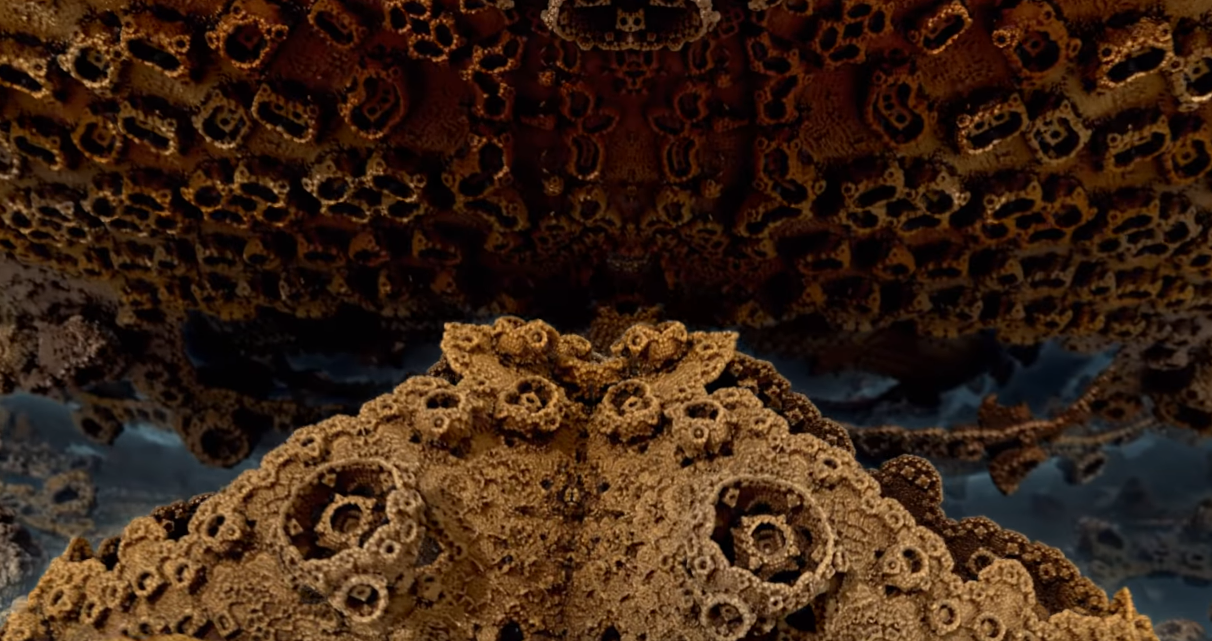
\includegraphics[scale=0.3]{cap1.PNG}
}
\end{figure}
\section{Discussion}




\end{document}
